\section{Week 9}

\textbf{\large \underline{Bode Plot Revision}}

Given an unity feedback closed loop system as $\frac{Y}{U}=\frac{G_c(j\omega)G_p(j\omega)}{1+G_c(j\omega)G_p(j\omega)}$,
\begin{itemize}
    \item $Y(j\omega)\to \infty$ if the following conditions are met:
    \begin{align*}
        \begin{cases}
            \angle G_c(j\omega)G_p(j\omega)=\pm 180^{\circ} \\
            |G_c(j\omega)G_p(j\omega)|=1
        \end{cases}
    \end{align*}
\end{itemize}
\textbf{\large \underline{Gain Margin (GM)}} 
\begin{itemize}
    \item GM $\eqdef$ the factor by which $|G_c(j\omega)G_p(j\omega)|$ must be multiplied for the result to reach 1 when $\angle G_c(j\omega)G_p(j\omega)=\pm 180^{\circ}$;
    \begin{equation*}
        \text{Gain Margin}\eqdef \frac{1}{|G_c(j\omega_c)G_p(j\omega_c)|}
    \end{equation*}
    \item Given open loop transfer function $G(s)$, how to find GM?
    \begin{enumerate}
        \item Find frequency where \textbf{PHASE} $=-180^{\circ}$;
        \item Find \textbf{GAIN} in dB at this \textbf{SAME FREQUENCY};
        \item $\textbf{GM} \eqdef 0 - \textbf{GAIN}$;
        \item $\textbf{GM}=\frac{1}{\bm{M}}$ where $\bm{M}=|G_c(j\omega)G_p(j\omega)|$ and $\textbf{Mag}=20\log_{10}(\bm{M})$.
    \end{enumerate}
\end{itemize}
\textbf{\large \underline{Phase Margin (PM)}} 
\begin{itemize}
    \item \textbf{PM} $\eqdef$ the phase angle when $|G(j\omega)|=1$ or $\textbf{GAIN} =0$ dB.  
    \item Given open loop transfer function $G(s)$, how to find PM?
    \begin{enumerate}
        \item Find frequency where \textbf{GAIN} $=0$ dB;
        \item Find \textbf{PHASE} in degs at this \textbf{SAME FREQUENCY};
        \item $\textbf{PM}\eqdef \textbf{PHASE} +180^{\circ}$.
    \end{enumerate}
    \item \textbf{Stability} As a rule of thumb, a phase margin of $\phi = 50^{\circ}$ is desirable. To achieve this, the Bode plot needs to maintain a -20dB/dec gradient both a decade before and after the cross-over frequency.
\end{itemize}
\begin{figure}[H]
    \centering
    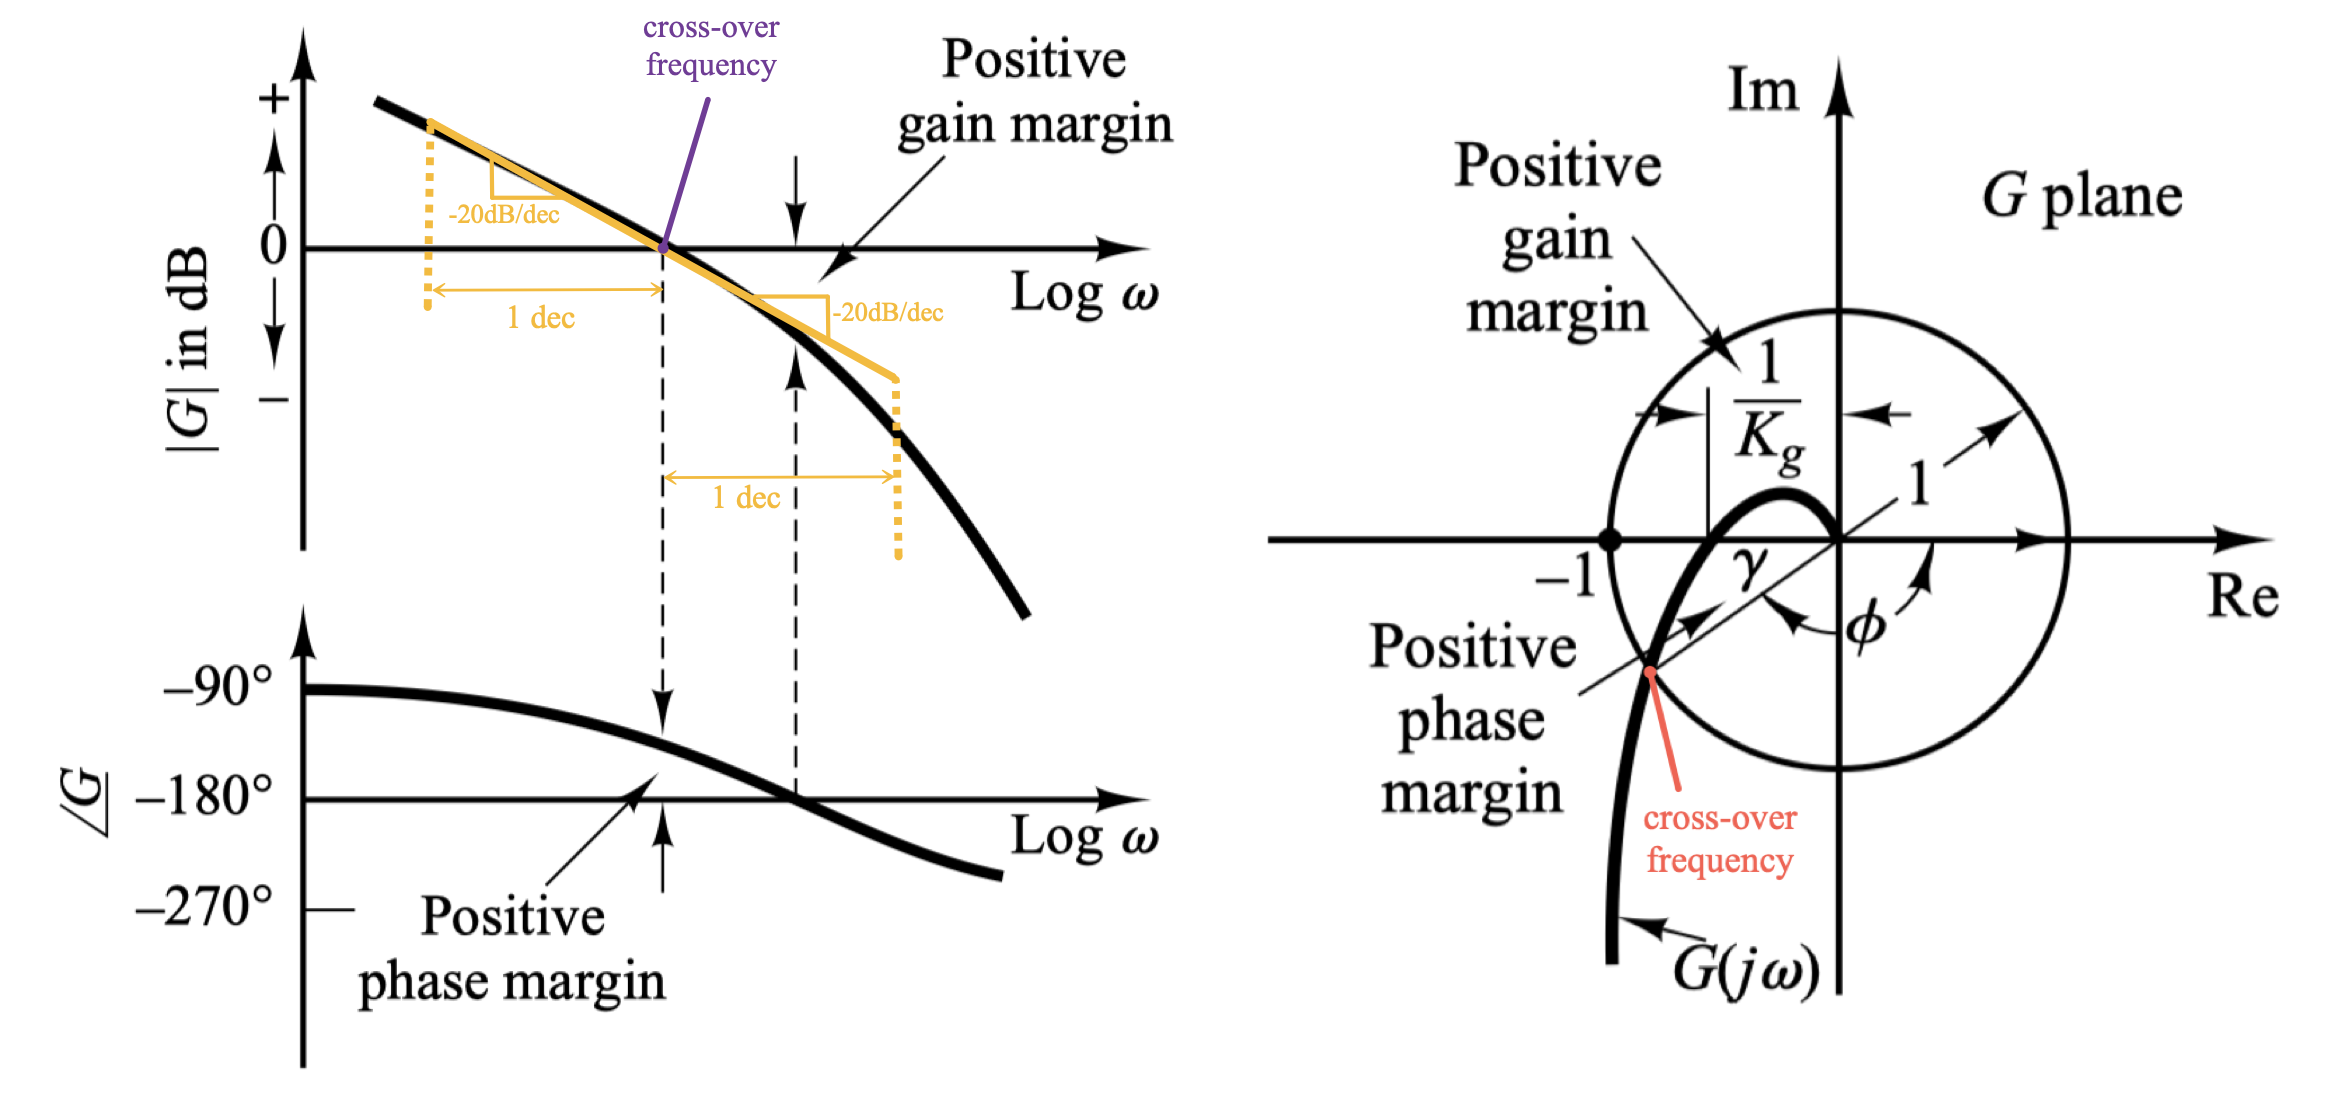
\includegraphics[width=1.0\linewidth]{images/phase_margin.png}
\end{figure}

\begin{itemize}
    \item \textbf{Cross-over frequency $\omega_c$:} the point on Nyquist plot that cuts the unit circle / the point on Bode plot that cuts the 0-dB line.
    \item A first order term with time constant $\tau$ has $\omega_c = \frac{1}{\tau}$.
\end{itemize}

\begin{table}[H]
\centering
\renewcommand{\arraystretch}{1.3}
\begin{tabular}{|c|c|c|c|}
\hline
\multicolumn{4}{|c|}{\textbf{Magnitude Plot}}                                                 \\ \hline
\multicolumn{2}{|c|}{\textbf{Poles}}                         & \textbf{Zeros} & \textbf{Gain} \\ \hline
$\frac{1}{\frac{s}{a}+1} \to \frac{1}{\frac{j\omega}{a}+1}$ &
  $\frac{1}{s}\to \frac{1}{j\omega}$ &
  Similar &
  \multirow{2}{*}{$\text{Mag}=20\log_{10}(K)$} \\ \cline{1-3}
$\because T=\frac{1}{a}\therefore \omega_c=a$ & $\omega_c=0$ & Similar        &               \\ \hline
\multicolumn{3}{|c|}{\begin{tabular}[c]{@{}c@{}}Turns on at $\omega_c$,\\ does not turn off\end{tabular}} &
  \begin{tabular}[c]{@{}c@{}}Turns on at $\omega = 0$,\\ does not turn off\end{tabular} \\ \hline
\multicolumn{2}{|c|}{\begin{tabular}[c]{@{}c@{}}-20 dB/dec\\ or -6 dB/oct\end{tabular}} &
  \begin{tabular}[c]{@{}c@{}}+20 dB/dec\\ or +6 dB/oct\end{tabular} &
  Const., no slope \\ \hline
\end{tabular}
\end{table}

\begin{table}[H]
\centering
\renewcommand{\arraystretch}{2}
\begin{tabular}{|c|c|c|c|c|}
\hline
\multirow{2}{*}{\textbf{Phase Plot}} & \multicolumn{2}{c|}{\textbf{Poles}}                     & \multicolumn{2}{c|}{\textbf{Zeros}}                 \\ \cline{2-5} 
                  & $\frac{1}{s+a}$   & $\frac{1}{s}$ & $s+a$            & $s$ \\ \hline
at $\omega=0.1 a$                    & $0^{\circ}$/dec & \multirow{3}{*}{$-90^{\circ}$ const.} & $0^{\circ}$/dec & \multirow{3}{*}{$90^{\circ}$/dec} \\ \cline{1-2} \cline{4-4}
in between        & $-45^{\circ}$/dec &               & $45^{\circ}$/dec &     \\ \cline{1-2} \cline{4-4}
at $\omega=10 a $ & $0^{\circ}$/dec   &               & $0^{\circ}$/dec  &     \\ \hline
\end{tabular}
\end{table}

\textbf{\large \underline{ZOH in Frequency Domain}}
\begin{itemize}
    \item Magnitude and phase contribution of ZOH \textbf{BY ITSELF}:
    \begin{align*}
        G_{ZOH} (s) &= \frac{T}{1+\frac{sT}{2}} \\
        |G_{ZOH}(j\omega)| &\approx T \\
        \angle G_{ZOH}(j\omega) &= \begin{cases}
            -\frac{\omega T}{2} & \text{(in rads)} \\
            -\frac{\omega T}{2} \color{red} \cdot \frac{180}{\pi} \color{black} & \text{(in degs)}
        \end{cases}
    \end{align*}
    \item Contribution of \textbf{ZOH + Sampler}:
    \begin{align*}
        G_{ZOH} (s) &= \frac{1}{1+\frac{sT}{2}} \\
        |G_{ZOH}(j\omega)| &\approx T \\
        \angle G_{ZOH}(j\omega) &= \begin{cases}
            -\frac{\omega T}{2} & \text{(in rads)} \\
            -\frac{\omega T}{2} \color{red} \cdot \frac{180}{\pi} \color{black} & \text{(in degs)}
        \end{cases}
    \end{align*}
    (because the sampler attenuates the signal by $\frac{1}{T}$)
    \item If a system is expected to let through signals up to $X$ Hz, then to avoid amplitude distortion caused by the ZOH, the sampling rates has to be $8X$ to $10X$ Hz, or even faster.
\end{itemize}


\textbf{\large \underline{Continuous-to-Discrete Conversion:}}
\begin{figure}[H]
    \centering
    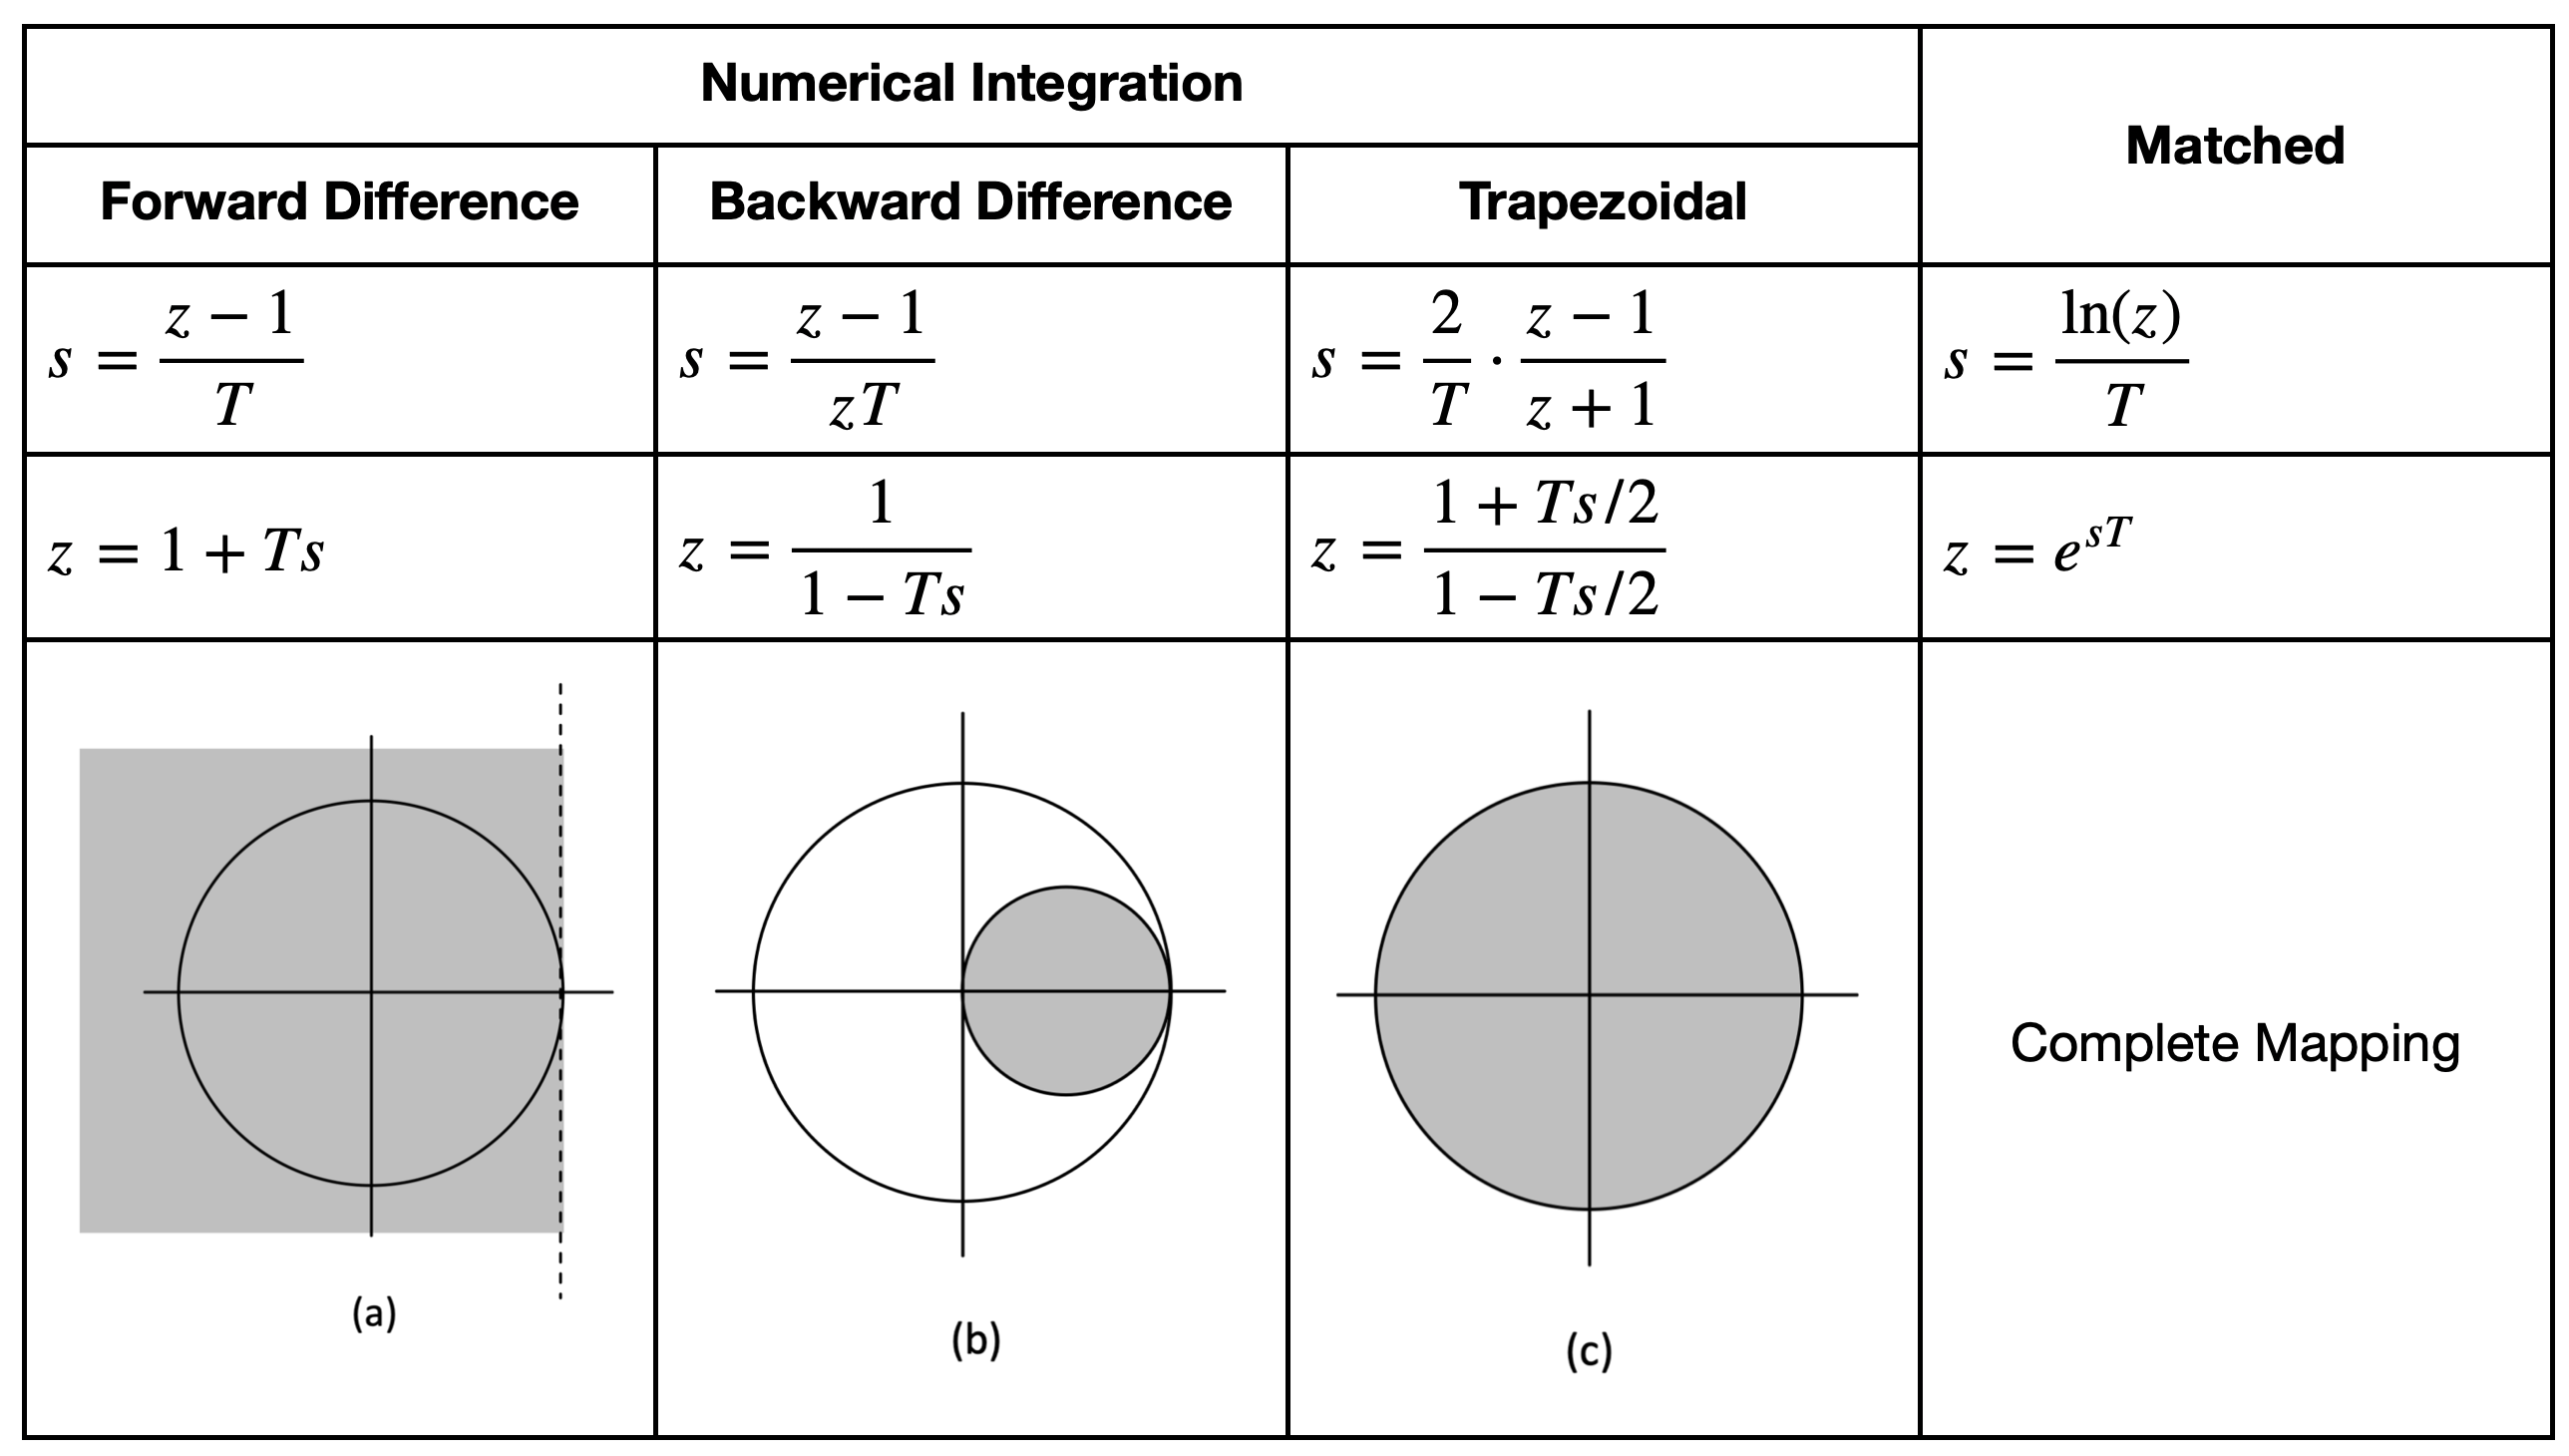
\includegraphics[width=1.0\linewidth]{images/z_s_mapping_table.png}
\end{figure}

\textbf{Important Remarks:}
\begin{itemize}
    \item If you're converting JUST the plant or the controller TF, DO NOT use 'c2d()' or 'c2dm()' as they automatically include the ZOH.
    \item Do-it-by-hand example: given that $G(s)=\frac{4}{s(s+4)}$, $T=0.02$ s, find its discrete equivalent using matched dynamics method.
    \begin{enumerate}
        \item 
    \end{enumerate}
\end{itemize}

\textbf{\large \underline{Disturbance Rejection:}}
\begin{itemize}
    \item Disturbances usually have lower frequencies.
    \item If $|G_{c}(j\omega_{dist}G_p(j\omega_{dist}))|\geq \frac{1}{\epsilon}$, then effect of disturbance is less than $\epsilon$.
    \begin{itemize}
        \item Example: Given the design that
        \begin{equation*}
            \left|\frac{C(j\omega)}{D(j\omega)}\right|\leq 0.01 \; \forall \; \omega \leq 0.1 \; \text{rad/s}\; ,
        \end{equation*}
        Find $|G_c(j\omega)G_p(j\omega)|$ at $\omega = 0.1$ rad/s.
        \begin{itemize}
            \item Solution:
            \begin{align*}
             |G_c(j\omega)G_p(j\omega)|&=20\log_{10}(\frac{1}{0.01}) \\
             &=40 \; \text{dB}
            \end{align*}
        \end{itemize}
    \end{itemize}
\end{itemize}

\textbf{\large \underline{Noise Rejection:}}
\begin{itemize}
    \item Noises usually have higher frequencies.
    \item If $|G_c(j\omega_{noise})G_p(j\omega_{noise})|\leq \epsilon$, then effect of noise is less than $\epsilon$.
    \begin{itemize}
        \item Example: Given the design that
        \begin{equation*}
            \left|\frac{C(j\omega)}{N(j\omega)}\right|\leq 0.001 \; \forall \; \omega \geq 100 \; \text{rad/s}\; ,
        \end{equation*}
        Find $|G_c(j\omega)G_p(j\omega)|$ at $\omega = 100$ rad/s.
        \begin{itemize}
            \item Solution:
            \begin{align*}
             |G_c(j\omega)G_p(j\omega)|&=20\log_{10}(0.001) \\
             &=-10 \; \text{dB}
            \end{align*}
        \end{itemize}
    \end{itemize}
\end{itemize}

\begin{figure}[H]
    \centering
    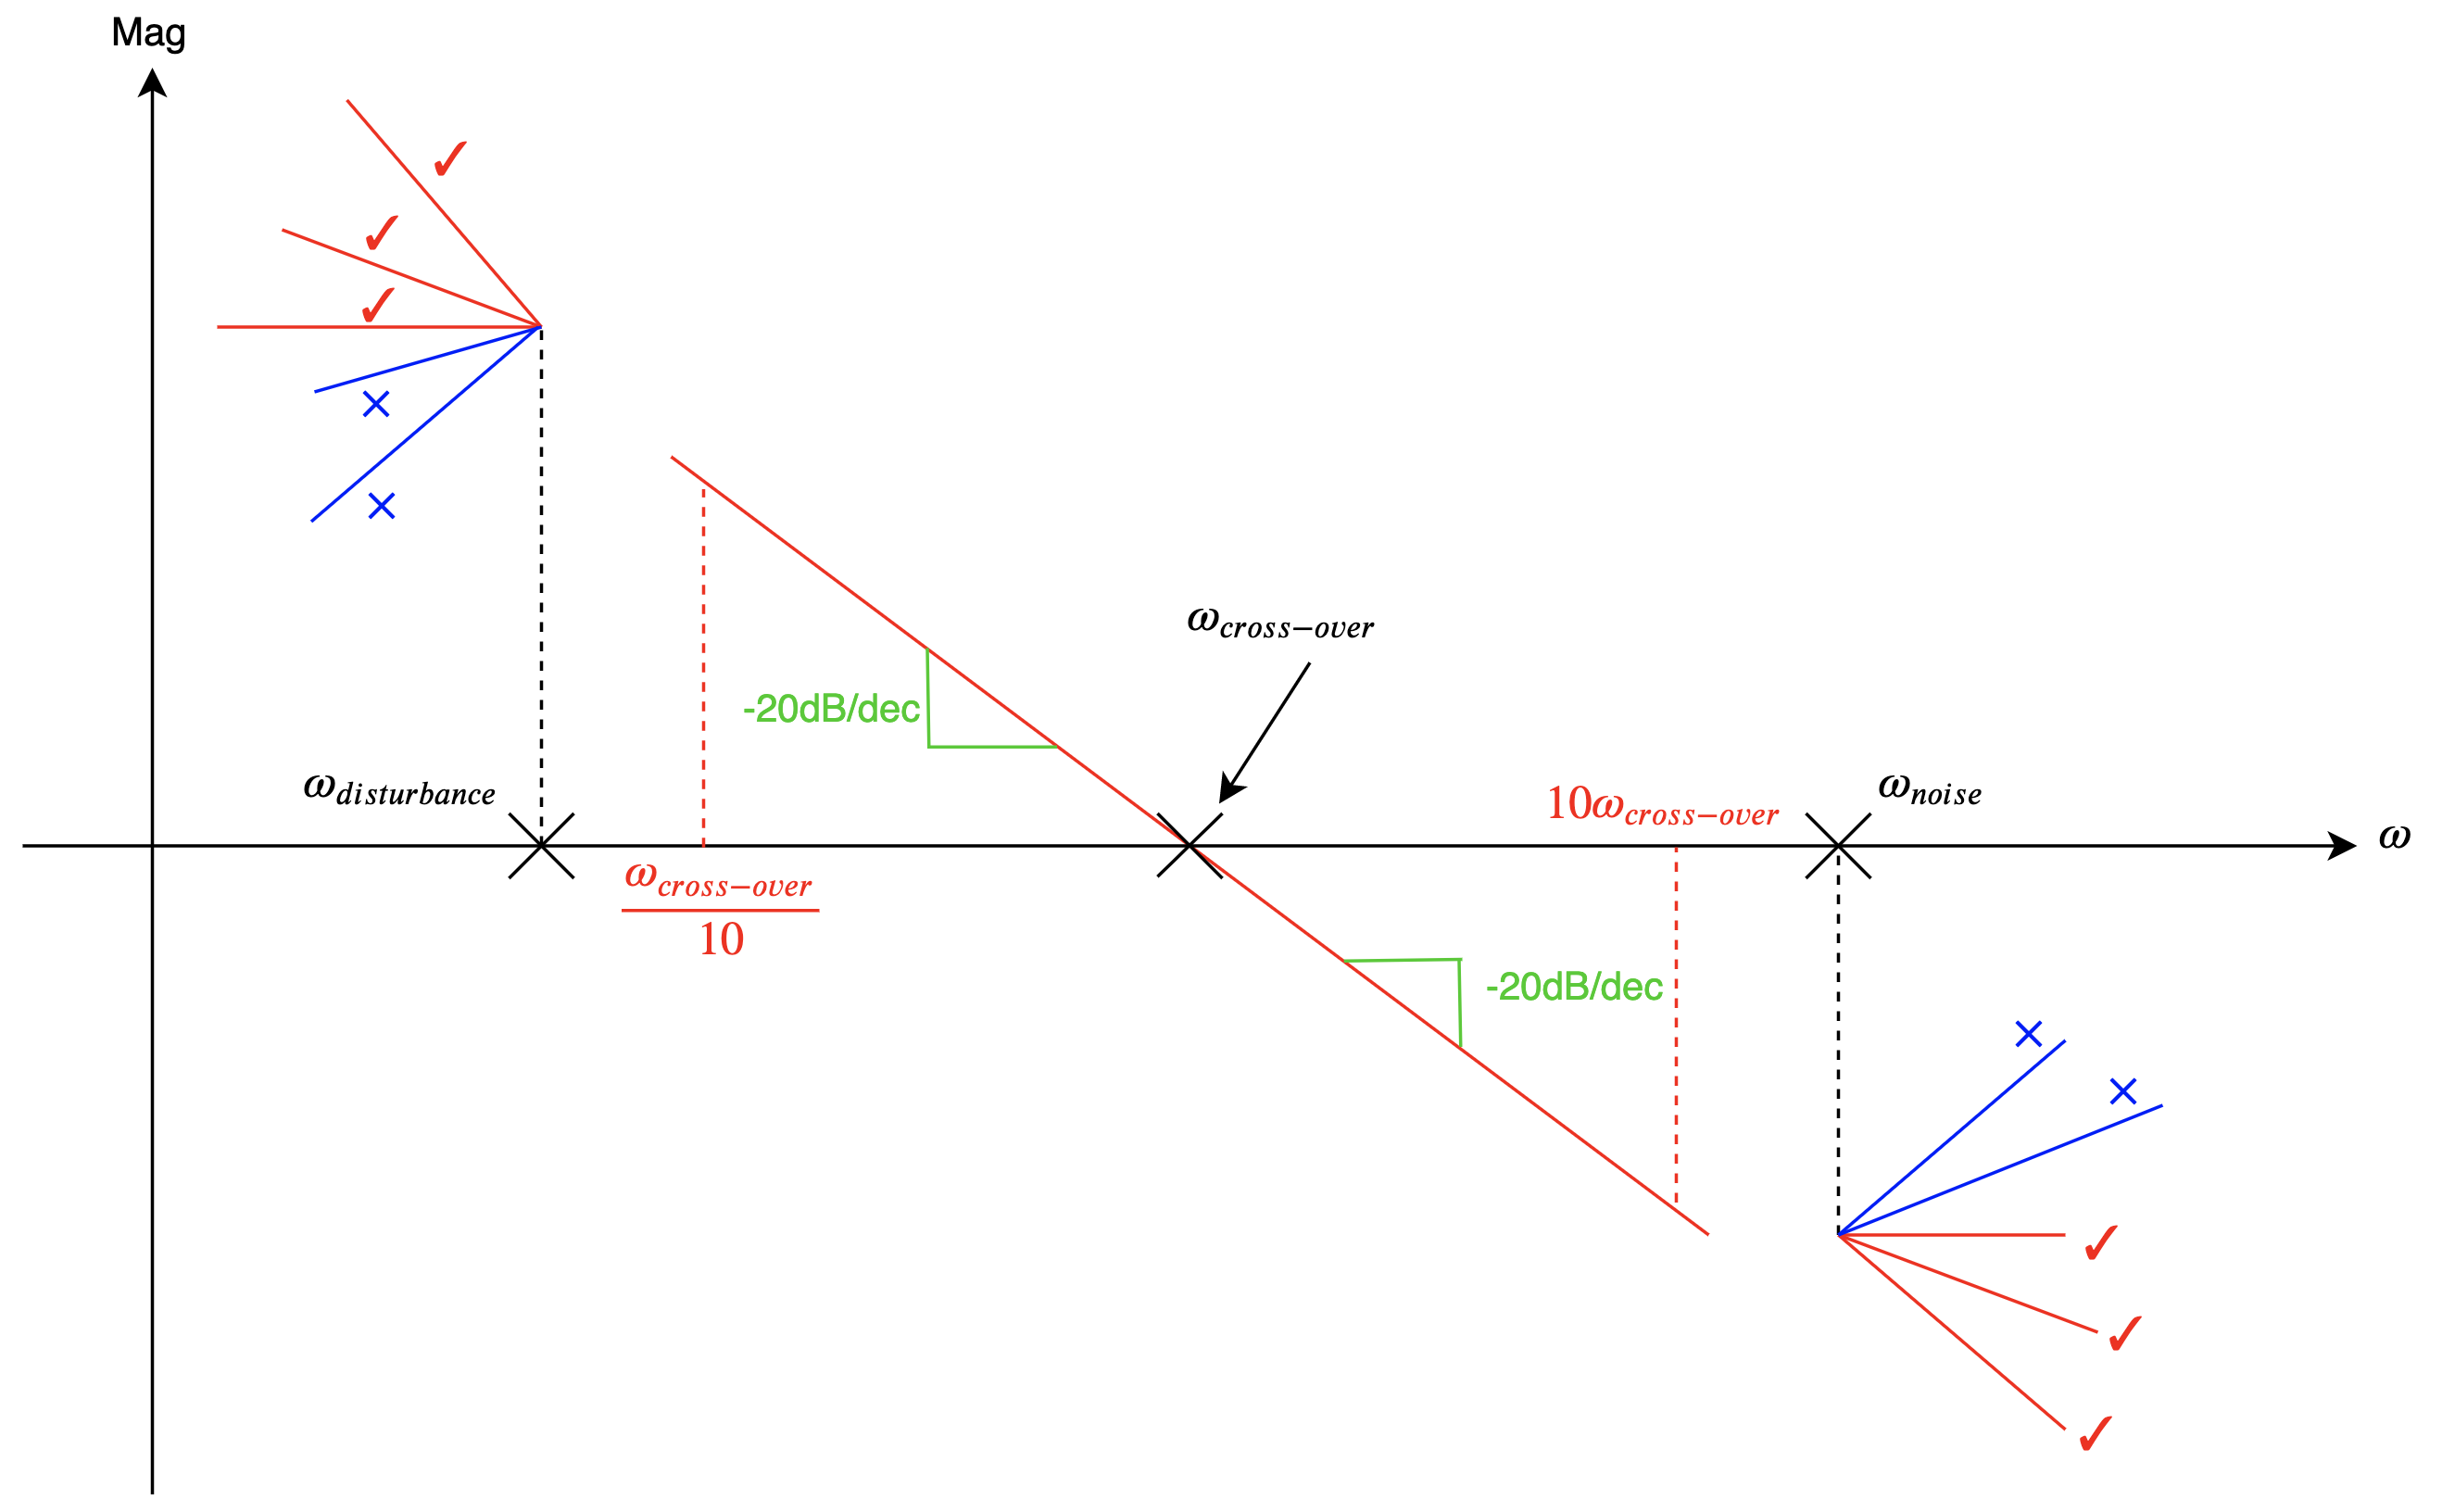
\includegraphics[width=1.0\linewidth]{images/Bode_rejection.png}
\end{figure}